\documentclass[12pt]{report}
\usepackage[utf8]{inputenc}
\usepackage[russian]{babel}
%\usepackage[14pt]{extsizes}
\usepackage{listings}
\usepackage{graphicx}
\usepackage{amsmath,amsfonts,amssymb,amsthm,mathtools} 

% Для листинга кода:
\lstset{ %
language=swift,                
basicstyle=\small\sffamily, % размер и начертание шрифта для подсветки кода
numbers=left,               % где поставить нумерацию строк (слева\справа)
numberstyle=\tiny,           % размер шрифта для номеров строк
stepnumber=1,                   % размер шага между двумя номерами строк
numbersep=5pt,                % как далеко отстоят номера строк от подсвечиваемого кода
showspaces=false,            % показывать или нет пробелы специальными отступами
showstringspaces=false,      % показывать или нет пробелы в строках
showtabs=false,             % показывать или нет табуляцию в строках
frame=single,              % рисовать рамку вокруг кода
tabsize=2,                 % размер табуляции по умолчанию равен 2 пробелам
captionpos=t,              % позиция заголовка вверху [t] или внизу [b] 
breaklines=true,           % автоматически переносить строки (да\нет)
breakatwhitespace=false, % переносить строки только если есть пробел
escapeinside={\#*}{*)}   % если нужно добавить комментарии в коде
}

% Для измененных титулов глав:
\usepackage{titlesec, blindtext, color} % подключаем нужные пакеты
\definecolor{gray75}{gray}{0.75} % определяем цвет
\newcommand{\hsp}{\hspace{20pt}} % длина линии в 20pt
% titleformat определяет стиль
\titleformat{\chapter}[hang]{\Huge\bfseries}{\thechapter\hsp\textcolor{gray75}{|}\hsp}{0pt}{\Huge\bfseries}


% plot
\usepackage{pgfplots}
\usepackage{filecontents}
\usetikzlibrary{datavisualization}
\usetikzlibrary{datavisualization.formats.functions}
\newenvironment{comment}{}{}
\begin{comment}
\begin{filecontents}{LevR.dat}
1 5928
2 16865
3 62333
4 372661
5 1909255
6 9065189
7 45325069
\end{filecontents}

\begin{filecontents}{LevT.dat}
1 3724258
2 7224736
3 12123365
4 16940041
5 23402008
6 32328258
7 30166031
\end{filecontents}

\begin{filecontents}{DamLevR.dat}
1 7456
2 21845
3 105445
4 407763
5 1966658
6 11002094
7 51219656
\end{filecontents}

\begin{filecontents}{DamLevT.dat}
1 4367560
2 8286833
3 12852145
4 18585284
5 24103230
6 27935583
7 30567571
\end{filecontents}
\end{comment}

\begin{document}
%\def\chaptername{} % убирает "Глава"
\begin{titlepage}
	\centering
	{\scshape\LARGE МГТУ им. Баумана \par}
	\vspace{3cm}
	{\scshape\Large Лабораторная работа №1\par}
	\vspace{0.5cm}	
	{\scshape\Large По курсу: "Анализ алгоритмов"\par}
	\vspace{1.5cm}
	{\huge\bfseries Расстояние Левенштейна\par}
	\vspace{2cm}
	\Large Работу выполнил: Саркисов Артём, ИУ7-53Б\par
	\vspace{0.5cm}
	\LargeПреподаватели:  Волкова Л.Л., Строганов Ю.В.\par

	\vfill
	\large \textit {Москва, 2020} \par
\end{titlepage}

\tableofcontents

\newpage
\chapter*{Введение}
\addcontentsline{toc}{chapter}{Введение}
\textbf{Расстояние Левенштейна} - минимальное количество операций вставки одного символа, удаления одного символа и замены одного символа на другой, необходимых для превращения одной строки в другую.

Расстояние Левенштейна применяется в теории информации и компьютерной лингвистике для:

\begin{itemize}
	\item исправления ошибок в слове(поисковая строка браузера)
	\item сравнения текстовых файлов утилитой diff
	\item в биоинформатике для сравнения генов, хромосом и белков
\end{itemize}

Целью данной лабораторной работы является изучение метода динамического программирования на материале алгоритмов
Левенштейна и Дамерау-Левенштейна. 

Задачами данной лабораторной являются:
\begin{enumerate}
  	\item изучение алгоритмов Левенштейна и Дамерау-Левенштейна нахождения расстояния между строками;
	\item применение метода динамического программирования для матричной реализации указанных алгоритмов; 
	\item получение практических навыков реализации указанных алгоритмов: двух алгоритмов в матричной версии и двух алгоритмов в рекурсивной версии; 
	\item сравнительный анализ линейной и рекурсивной реализаций выбранного алгоритма определения расстояния между строками по затрачиваемым ресурсам (времени и памяти); 
	\item экспериментальное подтверждение различий во временнóй эффективности рекурсивной и
нерекурсивной реализаций выбранного алгоритма определения расстояния между строками при
помощи разработанного программного обеспечения на материале замеров процессорного времени
выполнения реализации на варьирующихся длинах строк; 
	\item описание и обоснование полученных результатов в отчете о выполненной лабораторной
работе, выполненного как расчётно-пояснительная записка к работе. 
\end{enumerate}


\chapter{Аналитическая часть}
Задача по нахождению расстояния Левенштейна заключается в поиске минимального количества операций вставки/удаления/замены для превращения одной строки в другую.

При нахождении расстояния Дамерау — Левенштейна добавляется операция транспозиции (перестановки соседних символов).  
 
\textbf{Действия обозначаются так:} 
\begin{enumerate}
  	\item D (англ. delete) — удалить;
	\item I (англ. insert) — вставить;
	\item R (replace) — заменить;
	\item M(match) - совпадение;
\end{enumerate}

Пусть $S_{1}$ и $S_{2}$ — две строки (длиной M и N соответственно) над некоторым алфавитом, тогда расстояние Левенштейна можно подсчитать по следующей рекуррентной формуле (1.1):

\begin{equation}
D(i,j) = \left\{ \begin{array}{ll}
 0, & \textrm{$i = 0, j = 0$}\\
 i, & \textrm{$j = 0, i > 0$}\\
 j, & \textrm{$i = 0, j > 0$}\\
min(\\
D(i,j-1)+1,\\
D(i-1, j) +1, &\textrm{$j>0, i>0$}\\
D(i-1, j-1) + m(S_{1}[i], S_{2}[j])\\
),
  \end{array} \right.
\end{equation}

где $m(a,b)$ равна нулю, если $a=b$ и единице в противном случае; $min\{\,a,b,c\}$ возвращает наименьший из аргументов.

Расстояние Дамерау-Левенштейна вычисляется по следующей рекуррентной формуле (1.2):

\begin{equation}	    
D(i, j) =  \left\{
	\begin{aligned}
		&0, && i = 0, j = 0\\
		    	&i, && i > 0, j = 0\\
		    	&j, && i = 0, j > 0\\		    	
		    	&min \left\{
				\begin{aligned}
					&D(i, j - 1) + 1,\\
		            &D(i - 1, j) + 1,\\
		            &D(i - 1, j - 1) + m(S_{1}[i], S_{2}[i]), \\
		            &D(i - 2, j - 2) + m(S_{1}[i], S_{2}[i]),\\
		        \end{aligned} \right.
		        && 
				\begin{aligned}
					&, \text{ если } i, j > 0 \\
		            & \text{ и } S_{1}[i] = S_{2}[j - 1] \\
		            & \text{ и } S_{1}[i - 1] =  S_{2}[j] \\
		        \end{aligned} \\ 
		        &min \left\{
		        \begin{aligned}
		            &D(i, j - 1) + 1,\\
		            &D(i - 1, j) + 1, \\
		            &D(i - 1, j - 1) + m(S_{1}[i], S_{2}[i]),\\
		        \end{aligned} \right.  &&, \text{иначе}
			\end{aligned} \right.
\end{equation}
		\section{Вывод}
		В данном разделе были рассмотрены алгоритмы нахождения расстояния Левенштейна и Дамерау-Левенштейна, который является модификаций первого, учитывающего возможность перестановки соседних символов. 




\chapter{Конструкторская часть}
\textbf{Требования к программе:}
\begin{enumerate}
	\item На вход подаются две строки
	\item uppercase и lowercase буквы считаются разными
  	\item Две пустые строки - корректный ввод, программа не должна аварийно завершаться
  	\item Для всех алгоритмов выводиться процессорное время исполнения
  	\item Для всех алгоритмов кроме Левенштейна с рекурсивной реализацией должна выводиться матрица
\end{enumerate}
\section{Схемы алгоритмов}
В данной части будут рассмотрены схемы алгоритмов.

\begin{figure}[h]
\centering
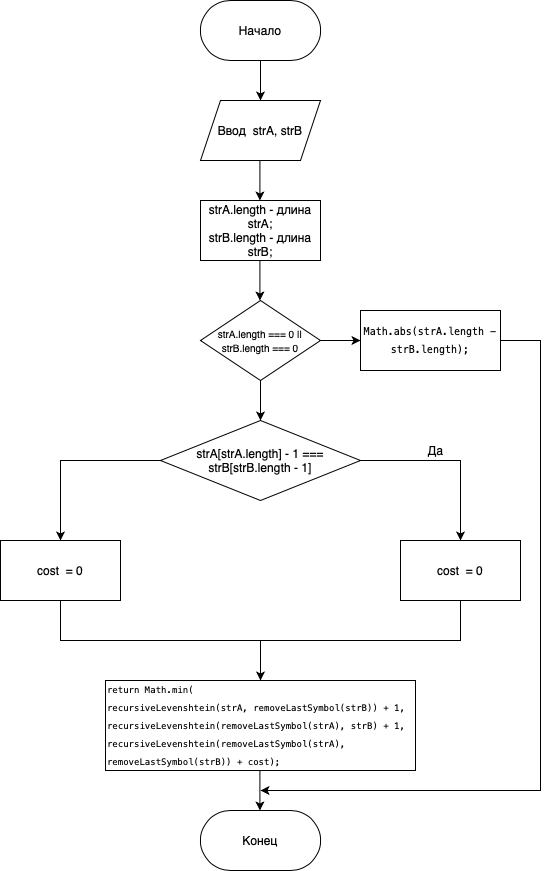
\includegraphics[width=0.70\linewidth]{recursiveLevenshtein.png}
\caption{Схема рекурсивного алгоритма нахождения расстояния Левенштейна}
\label{fig:mpr}
\end{figure}


\begin{figure}[h]
\centering
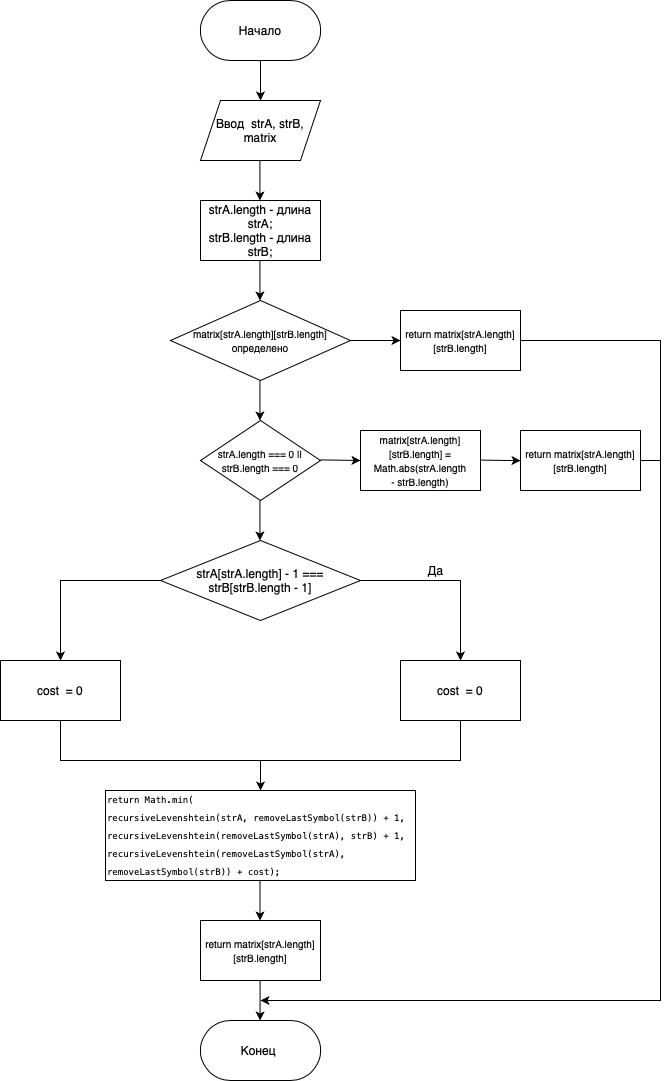
\includegraphics[width=0.70	\linewidth]{recursiveOptimizedLevenshtein.png}
\caption{Схема рекурсивного алгоритма нахождения расстояния Левенштейна с матричной оптимизацией}
\label{fig:mpr}
\end{figure}


\begin{figure}[h]
\centering
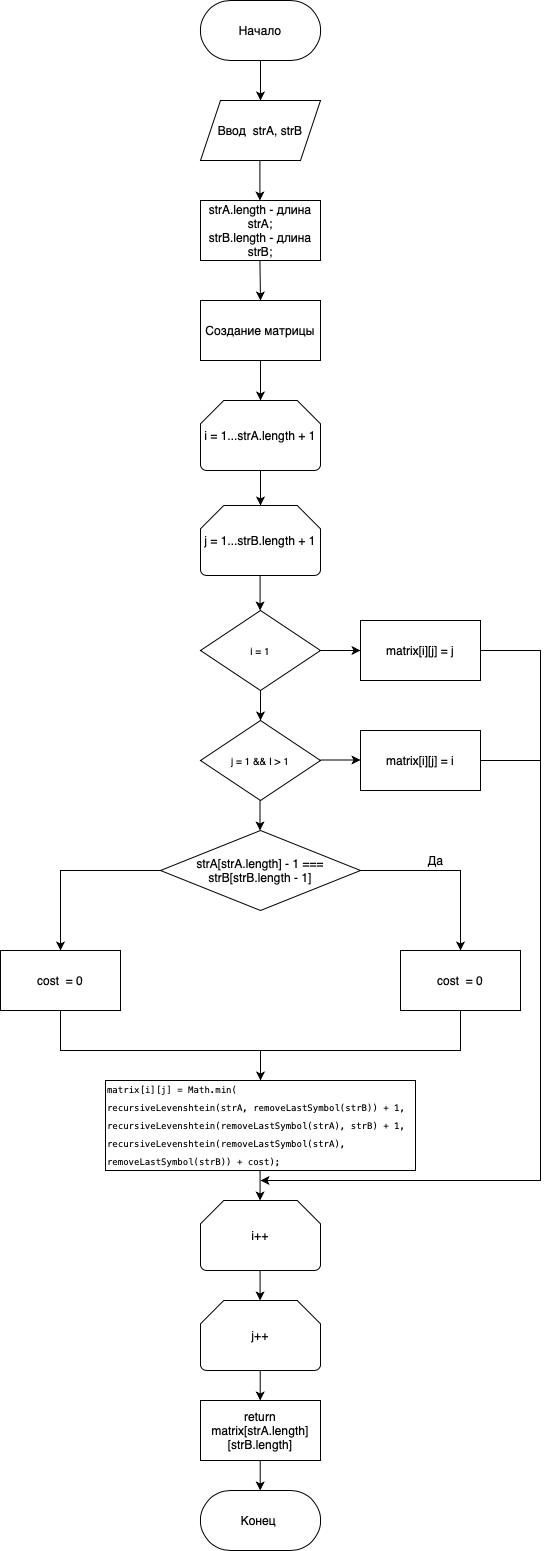
\includegraphics[width=0.40\linewidth]{matrixLevenshtein.png}
\caption{Схема матричного алгоритма нахождения расстояния Левенштейна}
\label{fig:mpr}
\end{figure}

\begin{figure}[h]
\centering
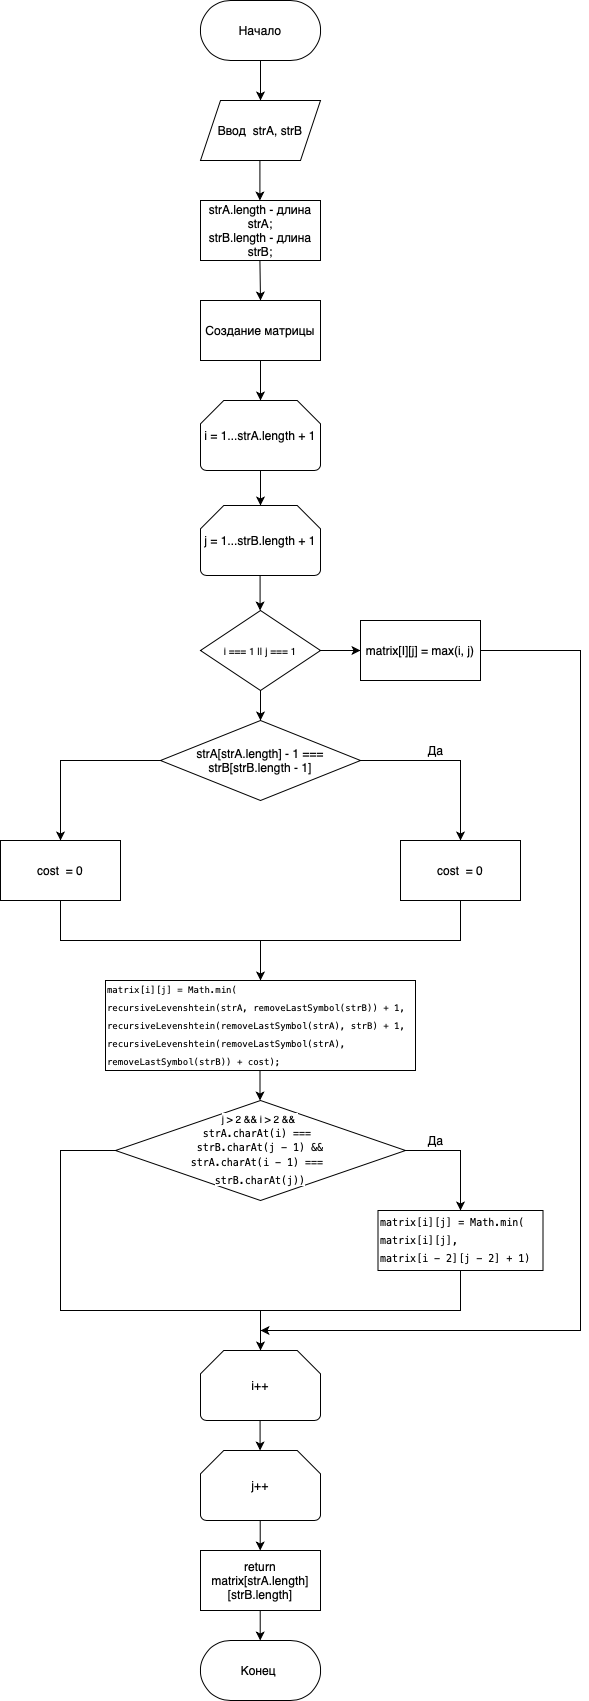
\includegraphics[width=0.40\linewidth]{matrixDamerauLevenshtein.png}
\caption{Схема матричного алгоритма нахождения расстояния Дамерау-Левенштейна}
\label{fig:mpr}
\end{figure}


\chapter{Технологическая часть}
\section{Выбор ЯП}
Для реализации программы был выбран язык программирования JavaScript в связи с потребностью практики разработки на нем. Среда разработки - VS Code.

\section{Реализация алгоритма}

\begin{lstlisting}[label=some-code,caption=Функция нахождения расстояния Левенштейна рекурсивно]
function recursiveLevenshtein(strA, strB) {
    if (strA.length === 0 || strB.length === 0) {
        return Math.abs(strA.length - strB.length);
    }
    let cost = (strA.charAt(strA.length - 1) === strB.charAt(strB.length - 1)) ? 0 : 1;
    return Math.min(recursiveLevenshtein(strA, removeLastSymbol(strB)) + 1,
                    recursiveLevenshtein(removeLastSymbol(strA), strB) + 1,
                    recursiveLevenshtein(removeLastSymbol(strA), removeLastSymbol(strB)) + cost);
}
\end{lstlisting}

\begin{lstlisting}[label=some-code,caption=Функция удаления последнего символа в строке]
function removeLastSymbol(str) {
    return str.slice(0, -1);
}
\end{lstlisting}

\begin{lstlisting}[label=some-code,caption=Функция нахождения расстояния Левенштейна рекурсивно с матрицей]
function recursiveOptimizedLevenshtein(strA, strB, matrix) {
    if (typeof(matrix[strA.length][strB.length]) !== 'undefined') {
        return matrix[strA.length][strB.length];
    } 
    if (strA.length === 0 || strB.length === 0) {
        matrix[strA.length][strB.length] = Math.abs(strA.length - strB.length);
        return matrix[strA.length][strB.length];
    }
    let cost = (strA.charAt(strA.length - 1) === strB.charAt(strB.length - 1)) ? 0 : 1;
    matrix[strA.length][strB.length] = Math.min(
        recursiveOptimizedLevenshtein(strA, removeLastSymbol(strB), matrix) + 1,
        recursiveOptimizedLevenshtein(removeLastSymbol(strA), strB, matrix) + 1,
        recursiveOptimizedLevenshtein(removeLastSymbol(strA), removeLastSymbol(strB), matrix) + cost);
    return matrix[strA.length][strB.length];
}
\end{lstlisting}


\begin{lstlisting}[label=some-code,caption=Функция нахождения расстояния Левенштейна матрично]
function matrixLevenshtein(strA, strB, matrix) {
    for (let i = 0; i < strA.length + 1; i++) {
        matrix[i] = [];
        for (let j = 0; j < strB.length + 1; j++) {
            if (i === 0) {
                matrix[i][j] = j;
            } else if(j === 0 && i > 0) {
                matrix[i][j] = i;
            } else {
                let cost = (strA.charAt(i - 1) === strB.charAt(j - 1)) ? 0 : 1;
                matrix[i][j] = Math.min(matrix[i][j - 1] + 1,
                                        matrix[i - 1][j] + 1,
                                        matrix[i - 1][j - 1] + cost);
            }
        }
    }
    return matrix[strA.length][strB.length];
}
\end{lstlisting}

\begin{lstlisting}[label=some-code,caption=Функция нахождения расстояния Дамерау-Левенштейна матрично]
function matrixDamerauLevenshtein(strA, strB, matrix) {
    for (let i = 0; i < strA.length + 1; i++) {
        matrix[i] = [];
        for (let j = 0; j < strB.length + 1; j++) {
            if (i === 0 || j === 0) {
                matrix[i][j] = Math.max(i, j);
            } else {
                let cost = (strA.charAt(i - 1) === strB.charAt(j - 1)) ? 0 : 1;
                matrix[i][j] = Math.min(matrix[i][j - 1] + 1,
                    matrix[i - 1][j] + 1,
                    matrix[i - 1][j - 1] + cost);
                if (j > 1 && i > 1 && 
                    strA.charAt(i) === strB.charAt(j - 1) && 
                    strA.charAt(i - 1) === strB.charAt(j)) {
                        matrix[i][j] = Math.min(matrix[i][j], matrix[i - 2][j - 2] + 1);
                }
            }
        }
    }
    return matrix[strA.length][strB.length];
}
\end{lstlisting}

\begin{lstlisting}[label=some-code,caption=Функция проверки транпозиции]
func isTransposition(_ strA: String, _ strB: String, _ i: Int, _ j: Int) -> Bool {
	return (strA[strA.index(strA.startIndex, offsetBy: i - 1)] == strB[strB.index(strB.startIndex, offsetBy: j  - 2)] &&
	strA[strA.index(strA.startIndex, offsetBy: i - 2)] == strB[strB.index(strB.startIndex, offsetBy: j - 1)])
}
\end{lstlisting}

\chapter{Исследовательская часть}

\section{Сравнительный анализ на основе замеров времени работы алгоритмов}

Был проведен замер времени работы каждого из алгоритмов.
\begin{table}
	\centering
	\caption{время исполнения в миллимекундах}
	\begin{tabular}{|c c c c c|} 
 	\hline
	len & Lev(R) & Lev(RM) & Lev(M) & DamLev(M) \\ [0.5ex] 
 	\hline\hline
  	1 & 0.025996 & 0.040448 & 0.022366 & 0.062549\\
 	\hline
 	2 & 0.048608 & 0.076069 & 0.033854 & 0.077381\\
 	\hline
	3 & 0.106327 & 0.085223 & 0.028715 & 0.076817\\
	\hline
	4 & 0.502248 & 0.080871 & 0.026586 & 0.073056\\
	\hline
	5 & 0.862543 & 0.079230 & 0.030535 & 0.080112.\\
	\hline
	6 & 0.653954 & 0.048213 & 0.019119 & 0.046017\\
	\hline
	7 & 2.383116 & 0.074804 & 0.026301 & 0.066106\\
	\hline
	8 & 5.957557 & 0.064507 & 0.021543 & 0.002099\\
	\hline
	9 & 21.236497 & 0.084806 & 0.030479 & 0.072075\\
	\hline
	10 & 112.217936 & 0.088567 & 0.041352 & 0.088084\\
	\hline
	\end{tabular}
\end{table}

\begin{tikzpicture}
\begin{axis}[
    	axis lines = left,
    	xlabel={len (symbols)},
    	ylabel={time (ticks)},
    	xmin=1, xmax=8,
    	ymin=1, ymax=500000,
	legend pos=north west,
	ymajorgrids=true
]
\addplot[color=red] table[x index=0, y index=1] {LevRecursive.dat}; 
\addplot[color=orange] table[x index=0, y index=1] {LevRecursiveMatr.dat};
\addplot[color=blue, mark=square] table[x index=0, y index=1] {LevMatr.dat};
\addplot[color=green, mark=square] table[x index=0, y index=1] {DamLevMatr.dat};

\addlegendentry{LevRec}
\addlegendentry{LevRecMatr}
\addlegendentry{LevMatr}
\addlegendentry{DamLevMatr}
\end{axis}
\end{tikzpicture}


\par
Наиболее эффективными по времени при маленькой длине слова являются рекурсивные реализации алгоритмов. Показатели рекурсивного алгоритма Левенштейна при увеличении размера слов резко ухудшаются. Это связано с большим количеством повторов. Рекурсивная версия с матрицей не теряет своей производительности так как там исключаются повторы. Время работы алгоритма, использующего матрицу, намного меньше благодаря тому, что в нем требуется только (m + 1)*(n + 1) операций заполнения ячейки матрицы. Также видно, что алгоритм Дамерау-Левенштейна работает немного дольше алгоритма Левенштейна, т.к. в нем добавлены дополнительные проверки, однако алгоритмы примерно одинаковы по временной эффективности.

\section{Тесты}

\par
Проведем тестирование программы. В столбцах "Ожидание" и "Результат" 4 числа соответсвуют рекурсивному алгоритму нахождения расстояния Левенштейна, рекурсивно-матричному алгоритму нахождения расстояния Левенштейна, матричному алгоритму расстояния Левенштейна, матричному алгоритму нахождения расстояния Дамерау-Левенштейна.

\begin{table} 
	\centering
	\caption{Таблица тестовых данных}
	\begin{tabular}{|c c c c c|} 
 	\hline
	№ & Слово №1 & Слово №2 & Ожидание & Результат \\ [0.8ex] 
 	\hline\hline
 	1 &  &  & 0 0 0 0 & 0 0 0 0\\
 	\hline
 	2 & 1234 & 2143 & 3 3 3 2 & 3 3 3 2\\
 	\hline
	3 & amm & add & 2 2 2 2 & 2 2 2 2\\
	\hline
	4 & error & dog & 4 4 4 4 & 4 4 4 4\\
	\hline
	5 &  & submission & 10 10 10 10 & 10 10 10 10\\
	\hline
	6 & mochombo & 0 & 8 8 8 8 & 8 8 8 8\\
	\hline
	7 & dfufdfd & fddfdffdd & 5 5 5 4  & 5 5 5 4\\
	\hline
	\end{tabular}
\end{table}



\chapter*{Заключение}
\addcontentsline{toc}{chapter}{Заключение}
Был изучен метод динамического программирования на материале алгоритмов Левенштейна и Дамерау-Левенштейна.
Также изучены алгоритмы Левенштейна и Дамерау-Левенштейна нахождения расстояния между строками, получены практические навыки раелизации указанных алгоритмов
в матричной  и рекурсивных версиях. 

Экспериментально было подтверждено различие во временной эффективности рекурсивной и нерекурсивной реализаций выбранного алгоритма определения расстояния между строками при помощи разработаного программного обеспечения на материале замеров процессорного времени выполнения реализации на варьирующихся длинах строк. 

В результате исследований делается вывод о том, что матричная реализация данных алгоритмов заметно выигрывает по времени при росте длины строк, следовательно более применима в реальных проектах.

\addcontentsline{toc}{chapter}{Литература}
\bibliographystyle{utf8gost705u}  % стилевой файл для оформления по ГОСТу
\nocite{*}
\bibliography{51-biblio}   % имя библиографической базы (bib-файла)

\end{document}
